\section{Results}\label{sec:results}

All numbers in this section are produced by \texttt{experiments/v13\_tables.py} and \texttt{experiments/v13\_figs.py} from the result files named in each table note. Differences are per-user paired differences of nDCG@10 multiplied by $10^{3}$, with the 95\% half-width in brackets. A comparison is called significant only when the Holm-adjusted p value is below 0.05 and the test is named. Tests are the per-user paired t test over the pooled test users (n = 22,612 on KuaiRand-27K) and the Nadeau-Bengio corrected resampled t test over the five split means (\citealp{nadeau2003}); the Holm family is stated in each table.

\subsection{Methods and search budgets}\label{sec:res-methods}

Table~\ref{tab:methods} lists the mean and standard deviation over the five splits. The search budgets differ by two orders of magnitude, so they are reported with every number. LEAF-LGN+DAX searches 3,840 configurations per split, the QP family with DAX 3,200, and the QP family itself 20. The budget of the fair baseline is therefore not matched in the strict sense; Section~\ref{sec:res-fair} discusses what this does to the comparison.

\begin{table}[tbp]
\centering
\footnotesize
\caption{Methods on KuaiRand-27K (temporal, all users): mean and standard deviation of nDCG@10 over the five splits, configurations searched per split, and the source file.}
\label{tab:methods}
\begin{adjustbox}{max width=\linewidth}
\begin{tabular}{lrrrr}
\toprule
Method & Mean & SD & Configurations & Source \\
\midrule
LEAF-LGN+DAX & 0.4854 & 0.0009 & 3840 & dax\_lgn\_post.json \\
LEAF-LGN (post-hoc run) & 0.4736 & 0.0002 & 12 & dax\_lgn\_post.json \\
LEAF-LGN (stored, v10) & 0.4728 & 0.0011 & 197 & leaf\_lgn.json \\
QP family & 0.4634 & 0.0031 & 20 & learned\_kuairand\_t\_qp.json \\
QP family+DAX & 0.4733 & 0.0012 & 3200 & dax\_qp.json \\
QP family (retrained) & 0.4652 & 0.0017 & 10 & dax\_qp.json \\
r-AdjNorm & 0.4620 & 0.0008 & 8 & learned\_kuairand\_t\_base.json \\
LightGCN & 0.4576 & 0.0031 & 4 & learned\_kuairand\_t\_base.json \\
LightGCN+DAX & \textnormal{\{TBD:results/v11/dax\_lightgcn.json LightGCN+DAX mean\}} & \textnormal{\{TBD:results/v11/dax\_lightgcn.json LightGCN+DAX sd\}} & \textnormal{\{TBD:results/v11/dax\_lightgcn.json LightGCN+DAX n\_configs\}} & \textnormal{\{TBD:results/v11/dax\_lightgcn.json LightGCN+DAX\}} \\
EASE & 0.4507 & 0.0009 & 27 & dax\_ease.json \\
EASE+DAX & 0.4623 & 0.0010 & 8640 & dax\_ease.json \\
DIN & 0.4675 & 0.0007 & 4 & din\_27k.json \\
DIN+DAX & 0.4796 & 0.0015 & 1280 & din\_27k.json \\
SIM & \textnormal{\{TBD:results/v12/sim\_27k.json SIM mean\}} & \textnormal{\{TBD:results/v12/sim\_27k.json SIM sd\}} & \textnormal{\{TBD:results/v12/sim\_27k.json SIM n\_configs\}} & \textnormal{\{TBD:results/v12/sim\_27k.json SIM\}} \\
SIM+DAX & \textnormal{\{TBD:results/v12/sim\_27k.json SIM+DAX mean\}} & \textnormal{\{TBD:results/v12/sim\_27k.json SIM+DAX sd\}} & \textnormal{\{TBD:results/v12/sim\_27k.json SIM+DAX n\_configs\}} & \textnormal{\{TBD:results/v12/sim\_27k.json SIM+DAX\}} \\
\bottomrule
\end{tabular}
\end{adjustbox}
\par\smallskip
\begin{minipage}{\linewidth}\raggedright\footnotesize Configurations: post-hoc runs count backbone trainings times DAX configurations times gammas. The stored LEAF-LGN counts another unit (not comparable). QP family is the per-split best of the three stored QP variants on validation.\end{minipage}
\end{table}


\subsection{Main comparison}\label{sec:res-main}

Table~\ref{tab:main} gives the paired comparisons of LEAF-LGN+DAX with each comparator of the main family. The family has seven members: the QP family, the QP family with DAX, the LEAF-LGN backbone without DAX, r-AdjNorm, LightGCN, DIN and DIN with DAX. SIM and SIM with DAX are part of the family but have no result file for KuaiRand-27K yet, so their rows are marked as pending and the Holm correction runs over the seven comparators present. EASE and EASE with DAX are reported outside the family. Table~\ref{tab:sens} shows that adding them to the family does not change any conclusion at the 0.05 level.

\begin{table}[tbp]
\centering
\footnotesize
\caption{Main results on KuaiRand-27K: LEAF-LGN+DAX against every comparator of the main family, with per-user and split-level (Nadeau-Bengio) tests.}
\label{tab:main}
\begin{adjustbox}{max width=\linewidth}
\begin{tabular}{lrccccc}
\toprule
Comparator & Mean & Diff.\ [95\% hw] & $p$ & $p_{\mathrm{Holm}}$ & NB $p$ & NB $p_{\mathrm{Holm}}$ \\
\midrule
LEAF-LGN+DAX (reference) & 0.4854 & n/a & n/a & n/a & n/a & n/a \\
\midrule
\multicolumn{7}{l}{Holm family: LEAF-LGN+DAX minus each comparator} \\
QP family & 0.4634 & +22.32 [1.83] & $3.64\times10^{-125}$ & $2.18\times10^{-124}$ & 0.023 & $4.56\times10^{-2}$ \\
QP family+DAX & 0.4733 & +12.04 [1.63] & $3.96\times10^{-47}$ & $7.92\times10^{-47}$ & 0.006 & $2.23\times10^{-2}$ \\
LEAF-LGN (post-hoc run) & 0.4736 & +11.96 [1.47] & $6.55\times10^{-57}$ & $1.97\times10^{-56}$ & 0.001 & $6.85\times10^{-3}$ \\
r-AdjNorm & 0.4620 & +23.79 [1.96] & $2.43\times10^{-123}$ & $1.22\times10^{-122}$ & 0.000 & $2.73\times10^{-4}$ \\
LightGCN & 0.4576 & +28.15 [1.86] & $5.33\times10^{-190}$ & $3.73\times10^{-189}$ & 0.008 & $2.44\times10^{-2}$ \\
DIN & 0.4675 & +18.26 [1.97] & $1.41\times10^{-73}$ & $5.62\times10^{-73}$ & 0.001 & $6.62\times10^{-3}$ \\
DIN+DAX & 0.4796 & +5.73 [1.64] & $7.95\times10^{-12}$ & $7.95\times10^{-12}$ & 0.043 & $4.56\times10^{-2}$ \\
SIM & \textnormal{\{TBD:results/v12/sim\_27k.json SIM mean\}} & \textnormal{\{TBD:results/v12/sim\_27k.json SIM paired difference\}} & \textnormal{\{TBD:results/v12/sim\_27k.json SIM\}} & \textnormal{\{TBD:results/v12/sim\_27k.json SIM\}} & \textnormal{\{TBD:results/v12/sim\_27k.json SIM\}} & \textnormal{\{TBD:results/v12/sim\_27k.json SIM\}} \\
SIM+DAX & \textnormal{\{TBD:results/v12/sim\_27k.json SIM+DAX mean\}} & \textnormal{\{TBD:results/v12/sim\_27k.json SIM+DAX paired difference\}} & \textnormal{\{TBD:results/v12/sim\_27k.json SIM+DAX\}} & \textnormal{\{TBD:results/v12/sim\_27k.json SIM+DAX\}} & \textnormal{\{TBD:results/v12/sim\_27k.json SIM+DAX\}} & \textnormal{\{TBD:results/v12/sim\_27k.json SIM+DAX\}} \\
\midrule
\multicolumn{7}{l}{Outside the family (raw p values only; not Holm-adjusted)} \\
EASE & 0.4507 & +35.24 [2.24] & $6.53\times10^{-205}$ & n/a & 0.000 & n/a \\
EASE+DAX & 0.4623 & +23.26 [1.98] & $1.52\times10^{-115}$ & n/a & 0.001 & n/a \\
\bottomrule
\end{tabular}
\end{adjustbox}
\par\smallskip
\begin{minipage}{\linewidth}\raggedright\footnotesize Per-user columns: paired t test over the pooled test users (n = 22612); Holm within the family, over the 7 comparators present; NB: Nadeau-Bengio corrected resampled t test over the five split means (fraction of validation users 0.3); Holm over the same family. Missing family members (shown as TBD): SIM, SIM+DAX. Differences are per-user means x1e-3 nDCG@10 with the 95\% half-width.\end{minipage}
\end{table}


\begin{table}[tbp]
\centering
\footnotesize
\caption{Sensitivity of the Holm adjustment: the main family extended by EASE and EASE+DAX (the family size is given in the column header and counts the comparators whose files exist).}
\label{tab:sens}
\begin{adjustbox}{max width=\linewidth}
\begin{tabular}{lrccc}
\toprule
Comparator & $p$ & $p_{\mathrm{Holm}}$ (family of $9$) & NB $p$ & NB $p_{\mathrm{Holm}}$ \\
\midrule
QP family & $3.64\times10^{-125}$ & $2.55\times10^{-124}$ & 0.023 & $4.56\times10^{-2}$ \\
QP family+DAX & $3.96\times10^{-47}$ & $7.92\times10^{-47}$ & 0.006 & $2.23\times10^{-2}$ \\
LEAF-LGN (post-hoc run) & $6.55\times10^{-57}$ & $1.97\times10^{-56}$ & 0.001 & $6.85\times10^{-3}$ \\
r-AdjNorm & $2.43\times10^{-123}$ & $1.46\times10^{-122}$ & 0.000 & $3.52\times10^{-4}$ \\
LightGCN & $5.33\times10^{-190}$ & $4.27\times10^{-189}$ & 0.008 & $2.44\times10^{-2}$ \\
DIN & $1.41\times10^{-73}$ & $5.62\times10^{-73}$ & 0.001 & $6.62\times10^{-3}$ \\
DIN+DAX & $7.95\times10^{-12}$ & $7.95\times10^{-12}$ & 0.043 & $4.56\times10^{-2}$ \\
SIM & \textnormal{\{TBD:results/v12/sim\_27k.json SIM paired test\}} & \textnormal{\{TBD:results/v12/sim\_27k.json SIM paired test\}} & \textnormal{\{TBD:results/v12/sim\_27k.json SIM paired test\}} & \textnormal{\{TBD:results/v12/sim\_27k.json SIM paired test\}} \\
SIM+DAX & \textnormal{\{TBD:results/v12/sim\_27k.json SIM+DAX paired test\}} & \textnormal{\{TBD:results/v12/sim\_27k.json SIM+DAX paired test\}} & \textnormal{\{TBD:results/v12/sim\_27k.json SIM+DAX paired test\}} & \textnormal{\{TBD:results/v12/sim\_27k.json SIM+DAX paired test\}} \\
EASE & $6.53\times10^{-205}$ & $5.88\times10^{-204}$ & 0.000 & $1.16\times10^{-3}$ \\
EASE+DAX & $1.52\times10^{-115}$ & $7.61\times10^{-115}$ & 0.001 & $5.39\times10^{-3}$ \\
\bottomrule
\end{tabular}
\end{adjustbox}
\par\smallskip
\begin{minipage}{\linewidth}\raggedright\footnotesize The Holm values differ from Table~\ref{tab:main} only through the family size.\end{minipage}
\end{table}


The per-user paired test gives an adjusted p value below $10^{-11}$ for each of the seven comparators, and the sign is the same in every split for each of them (Figure~\ref{fig:forest}). The split-level test is also below 0.05 after Holm adjustment for all seven comparators, but the margins are small for the two QP comparators and for DIN with DAX, whose adjusted Nadeau-Bengio p values are $4.56\times10^{-2}$, $2.23\times10^{-2}$ and $4.56\times10^{-2}$. With five splits the split-level test has low power, and these values are the closest to the threshold in the paper.

\begin{figure}[tbp]
\centering
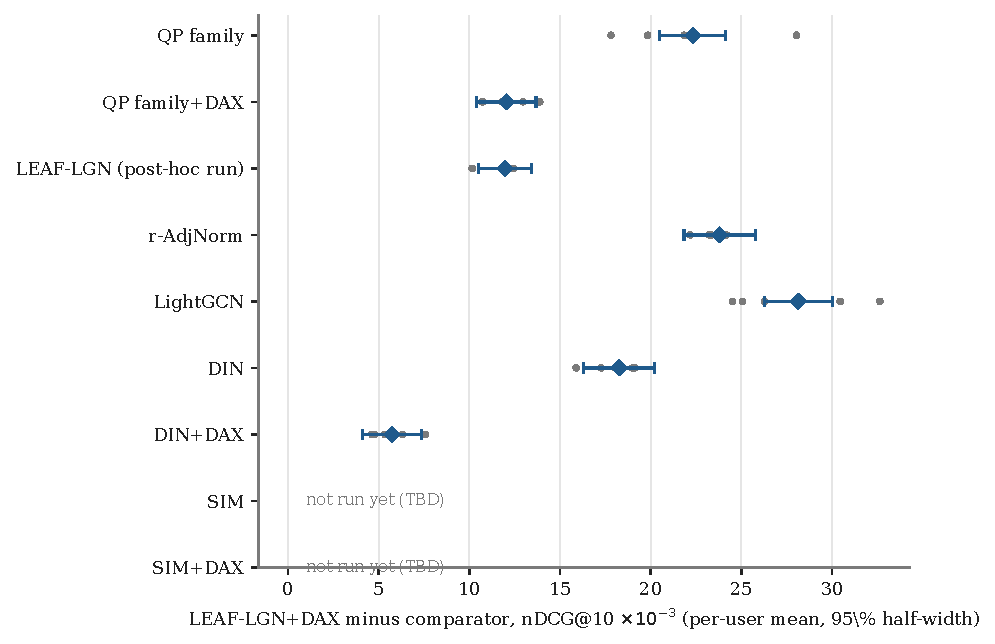
\includegraphics[width=0.85\linewidth]{figs/fig_forest.pdf}
\caption{Paired differences of LEAF-LGN+DAX against each comparator of the main family. Grey dots: the five split differences. Diamond: pooled per-user mean with its 95\% half-width. Source: \texttt{results/v11/dax\_lgn\_post.json} and the comparator files named in Table~\ref{tab:methods}.}
\label{fig:forest}
\end{figure}

The pre-declared gate for the primary comparison requires a paired difference of at least $15\times10^{-3}$ against the QP family, with both adjusted p values below 0.05 (\texttt{results/v11/stageB.txt}, Section 3). The observed difference is $+22.32$ [1.83], and the gate is passed. The gate was declared before Stage B, and the combination it evaluates is the post-hoc one described in the method section.

\subsection{Fair-baseline reading}\label{sec:res-fair}

The QP family has the smaller search budget, so the fairer reference for the DAX module is the QP family with DAX, which searches the QP backbones selected without DAX. Against that baseline LEAF-LGN+DAX is higher by $+12.04$ [1.63] (per-user t test, Holm-adjusted $p=7.92\times10^{-47}$; Nadeau-Bengio Holm-adjusted $p=2.23\times10^{-2}$). The DAX increment on the QP backbone is $+10.28$ [1.37] with an unadjusted Nadeau-Bengio p of 0.105, so on the split-level test the increment on the QP backbone alone is not significant. The LEAF backbone without DAX, against the stored QP family, is $+9.63$ [1.60] with an unadjusted Nadeau-Bengio p of 0.063; in the stage 1 run this comparison is not significant after Holm adjustment (Table~\ref{tab:fair}). The LEAF backbone is therefore not, by itself, a clear improvement over the QP family on the split-level test; the combination is.

\begin{table}[tbp]
\centering
\footnotesize
\caption{Fair-baseline reading: the DAX increments and the stored LEAF-LGN against the QP family, with their search budgets (configurations of the first and second method).}
\label{tab:fair}
\begin{adjustbox}{max width=\linewidth}
\begin{tabular}{lccccl}
\toprule
Comparison & Configurations & Diff.\ [95\% hw] & $p$ & NB $p$ & Test family \\
\midrule
LEAF-LGN+DAX minus QP family+DAX (fair baseline) & 3840 / 3200 & +12.04 [1.63] & $3.96\times10^{-47}$ & 0.006 & main family \\
QP family+DAX minus QP family (DAX on the QP backbone) & 3200 / 20 & +10.28 [1.37] & $1.09\times10^{-48}$ & 0.105 & raw \\
LEAF-LGN+DAX minus LEAF-LGN (DAX on the LEAF backbone) & 3840 / 12 & +11.96 [1.47] & $6.55\times10^{-57}$ & 0.001 & main family \\
LEAF-LGN (stored, v10) minus QP family & 197 / 20 & +9.63 [1.60] & $6.77\times10^{-32}$ & 0.063 & raw \\
\bottomrule
\end{tabular}
\end{adjustbox}
\par\smallskip
\begin{minipage}{\linewidth}\raggedright\footnotesize Rows marked raw are not Holm-adjusted: the stored v10 comparison is part of a different family (eight comparisons in the stage 1 run), and the DAX increments are reported beside the main family. The QP family + DAX search uses only the QP backbone configurations selected without DAX.\end{minipage}
\end{table}


\subsection{DAX on other backbones}\label{sec:res-backbone}

Table~\ref{tab:backbone} applies the same post-hoc DAX module to four backbones with a result file. The increments are $+11.98$ [1.64] for EASE (unadjusted Nadeau-Bengio p 0.000), $+10.28$ [1.37] for the QP family, $+11.96$ [1.47] for LEAF-LGN and $+12.53$ [1.41] for DIN. The LightGCN increment is pending (\url{results/v11/dax_lightgcn.json} is missing), and so is the SIM increment. The increment is positive on every backbone with a result, which is the basis for describing the module as backbone-agnostic. The claim is about the module's increment under the same post-hoc rule, not about the backbones' absolute accuracy.

\begin{table}[tbp]
\centering
\footnotesize
\caption{DAX is backbone-agnostic: nDCG@10 without and with the post-hoc DAX module on KuaiRand-27K, paired difference x1e-3 with the 95\% half-width, two-sided t test and the Nadeau-Bengio test over the split means.}
\label{tab:backbone}
\begin{adjustbox}{max width=\linewidth}
\begin{tabular}{lrcccc}
\toprule
Backbone & Without DAX & With DAX & Diff.\ [95\% hw] & $p$ & NB $p$ \\
\midrule
EASE & 0.4507 & 0.4623 & +11.98 [1.64] & $2.27\times10^{-46}$ & 0.000 \\
LightGCN & 0.4576 & \textnormal{\{TBD:results/v11/dax\_lightgcn.json LightGCN+DAX mean\}} & \textnormal{\{TBD:results/v11/dax\_lightgcn.json LightGCN+DAX minus results/v10/learned\_kuairand\_t\_base.json LightGCN paired difference\}} &  &  \\
QP family (stored) & 0.4634 & 0.4733 & +10.28 [1.37] & $1.09\times10^{-48}$ & 0.105 \\
LEAF-LGN (post-hoc run) & 0.4736 & 0.4854 & +11.96 [1.47] & $6.55\times10^{-57}$ & 0.001 \\
DIN & 0.4675 & 0.4796 & +12.53 [1.41] & $1.30\times10^{-67}$ & 0.011 \\
SIM & \textnormal{\{TBD:results/v12/sim\_27k.json SIM mean\}} & \textnormal{\{TBD:results/v12/sim\_27k.json SIM+DAX mean\}} & \textnormal{\{TBD:results/v12/sim\_27k.json SIM+DAX minus SIM paired difference\}} &  &  \\
\bottomrule
\end{tabular}
\end{adjustbox}
\par\smallskip
\begin{minipage}{\linewidth}\raggedright\footnotesize Raw p values (no family). The QP row uses the stored QP family as the reference, as in the fair-baseline reading.\end{minipage}
\end{table}


\subsection{Ablations of DAX}\label{sec:res-ablate}

Table~\ref{tab:ablate} decomposes the DAX module. The arms are run in a reduced setting: two backbone trainings, five gammas and an epoch window of three around the main selection. The full arm reproduces the per-split values of the main run, so the arms can be compared with each other. The gain of each arm is measured against the LEAF-LGN base of that run, which has a mean of 0.4706; this base is lower than the 0.4736 of the main run, so the gains in Table~\ref{tab:ablate} are larger than the main increment of $+11.96$ [1.47]. The comparisons that do not depend on the base are the differences from the full arm, in the rightmost columns.

Each removal lowers the score. Removing the examination factor $\kappa_t$ costs $+1.51$ [0.79] (Holm-adjusted $p=2.02\times10^{-4}$ by the per-user t test), removing the lifelong prior on $\theta_u$ costs $+1.78$ [0.61] ($p_{\text{Holm}}=2.16\times10^{-8}$), and removing the tag prior on $\alpha_i$ costs $+3.41$ [0.99] ($p_{\text{Holm}}=4.79\times10^{-11}$). Replacing the multiplicative form by the additive logit with tab effects costs $+6.09$ [0.96], which is the largest of the structural comparisons ($p_{\text{Holm}}=5.43\times10^{-35}$); the additive arm keeps 59.7\% of the full gain.

The shuffle controls test the item-level part of $\alpha_i$. Permuting $\alpha$ across all items removes the whole gain: the pooled shuffled arm has a gain of $-0.27$ [0.36], that is $-1.8\%$ of the full gain, and the full arm is higher by $+15.36$ [1.40] ($p_{\text{Holm}}=3.53\times10^{-101}$). Permuting $\alpha$ within each tag keeps 41.6\% of the full gain ($+6.28$ [1.10]), and the full arm is higher by $+8.81$ [1.00] ($p_{\text{Holm}}=2.47\times10^{-65}$). The within-tag arm therefore keeps a substantial part of the gain, which is the tag mean, and the remaining part lies in the item-level deviation from it. The three permutation seeds give the same ordering (Table~\ref{tab:ablate}, lower block): the across-item shuffles have gains between $-0.44$ and $-0.16$ and the within-tag shuffles between $+5.66$ and $+6.84$.

\begin{table}[tbp]
\centering
\footnotesize
\caption{DAX ablations on KuaiRand-27K (post-hoc): gain over the backbone of the ablation run, the difference to full DAX, and the shuffle controls.}
\label{tab:ablate}
\begin{adjustbox}{max width=\linewidth}
\begin{tabular}{lrcccccc}
\toprule
Arm & Configs & Mean & Gain [95\% hw] & $p_{\mathrm{Holm}}$ & Kept (\%) & Full minus arm & $p_{\mathrm{Holm}}$ \\
\midrule
full DAX & 320 & 0.4854 & +15.10 [1.42] & $8.82\times10^{-95}$ & 100.0 & n/a & n/a \\
no examination factor kappa\_t & 160 & 0.4839 & +13.59 [1.43] & $1.28\times10^{-76}$ & 90.0 & +1.51 [0.79] & $2.02\times10^{-4}$ \\
no lifelong prior on theta\_u & 160 & 0.4836 & +13.31 [1.43] & $7.92\times10^{-73}$ & 88.2 & +1.78 [0.61] & $2.16\times10^{-8}$ \\
no tag prior on alpha\_i & 160 & 0.4820 & +11.68 [1.22] & $1.28\times10^{-76}$ & 77.4 & +3.41 [0.99] & $4.79\times10^{-11}$ \\
additive logit (MRP-style), tab effects & 320 & 0.4794 & +9.01 [1.25] & $9.20\times10^{-45}$ & 59.7 & +6.09 [0.96] & $5.43\times10^{-35}$ \\
alpha shuffled across items & 960 & 0.4704 & -0.27 [0.36] & $1.48\times10^{-1}$ & -1.8 & +15.36 [1.40] & $3.53\times10^{-101}$ \\
alpha shuffled within tag & 960 & 0.4768 & +6.28 [1.10] & $1.23\times10^{-28}$ & 41.6 & +8.81 [1.00] & $2.47\times10^{-65}$ \\
\midrule
\multicolumn{8}{l}{Permutation seeds (pooled arm above selects over seeds; separate runs below)} \\
alpha shuffled across items, seed 0 &  &  & -0.44 [0.50] & NB 0.510 & -2.9 &  &  \\
alpha shuffled across items, seed 1 &  &  & -0.16 [0.53] & NB 0.986 & -1.0 &  &  \\
alpha shuffled across items, seed 2 &  &  & -0.20 [0.51] & NB 0.775 & -1.3 &  &  \\
alpha shuffled within tag, seed 0 &  &  & +5.66 [1.14] & NB 0.010 & 37.5 &  &  \\
alpha shuffled within tag, seed 1 &  &  & +6.84 [1.13] & NB 0.002 & 45.3 &  &  \\
alpha shuffled within tag, seed 2 &  &  & +6.35 [1.24] & NB 0.001 & 42.1 &  &  \\
\bottomrule
\end{tabular}
\end{adjustbox}
\par\smallskip
\begin{minipage}{\linewidth}\raggedright\footnotesize Gain: arm minus the LEAF-LGN base of the ablation run (mean 0.4706, 2 backbone trainings, five gammas, epoch window of 3 around the main selection). Full DAX reproduces the main run's splits. Holm within the seven gains (column p Holm); the column of full minus arm is Holm-adjusted within the six ablated arms. Kept: the arm's gain as a percentage of the full gain. Pooled shuffle entries select the permutation seed on validation.\end{minipage}
\end{table}


\subsection{KuaiRand-1K replication}\label{sec:res-1k}

Table~\ref{tab:1k} repeats the primary comparisons on KuaiRand-1K, which contains 842 test users pooled over the five splits. LEAF-LGN+DAX reaches 0.4590 against 0.4246 for the QP family, a difference of $+37.58$ [11.10] (per-user t test, Holm-adjusted $p=1.61\times10^{-10}$; Nadeau-Bengio Holm-adjusted $p=2.28\times10^{-2}$), and against 0.4358 for the QP family with DAX, a difference of $+25.82$ [9.66] (Holm-adjusted $p=3.91\times10^{-7}$; Nadeau-Bengio Holm-adjusted $p=2.18\times10^{-2}$). The DAX increment on the QP backbone, $+11.76$ [8.54], is significant under the per-user t test (Holm-adjusted $p=7.04\times10^{-3}$) but not under the split-level test (Nadeau-Bengio Holm-adjusted $p=0.160$). The 1K replication uses a wider QP search for the DAX arm (6,400 configurations against 3,200 at 27K), which favours the baseline. The 1K users are a subset of the 27K users, so the replication has lower power and is not an independent sample.

\begin{table}[tbp]
\centering
\footnotesize
\caption{KuaiRand-1K replication: LEAF-LGN+DAX against the QP family with and without DAX (nDCG@10).}
\label{tab:1k}
\begin{adjustbox}{max width=\linewidth}
\begin{tabular}{lrrrccccc}
\toprule
Method or comparison & Mean & SD & Configs & Diff.\ [95\% hw] & $p$ & $p_{\mathrm{Holm}}$ & NB $p$ & NB $p_{\mathrm{Holm}}$ \\
\midrule
LEAF-LGN+DAX & 0.4590 & 0.0038 & 3840 &  &  &  &  &  \\
QP family & 0.4246 & 0.0043 & 20 &  &  &  &  &  \\
QP family+DAX & 0.4358 & 0.0035 & 6400 &  &  &  &  &  \\
\midrule
LEAF-LGN+DAX minus QP family &  &  &  & +37.58 [11.10] & $5.37\times10^{-11}$ & $1.61\times10^{-10}$ & 0.011 & $2.28\times10^{-2}$ \\
LEAF-LGN+DAX minus QP family+DAX &  &  &  & +25.82 [9.66] & $1.96\times10^{-7}$ & $3.91\times10^{-7}$ & 0.007 & $2.18\times10^{-2}$ \\
QP family+DAX minus QP family &  &  &  & +11.76 [8.54] & $7.04\times10^{-3}$ & $7.04\times10^{-3}$ & 0.160 & $1.60\times10^{-1}$ \\
\bottomrule
\end{tabular}
\end{adjustbox}
\par\smallskip
\begin{minipage}{\linewidth}\raggedright\footnotesize KuaiRand-1K: 842 test users pooled over five splits (each split 30\% validation, 70\% test); 1K users are a subset of the 27K users, a lower-power replication. The 1K QP family + DAX arm searches all 20 QP configurations (6400 configurations in total) whereas the 27K arm searches the 10 selected ones (3200); this favours the baseline and is stated as such. Holm over the three comparisons of this table; NB over the split means. Split differences (x1e-3): LEAF-LGN+DAX minus QP family: +36.7 +25.7 +35.6 +37.2 +36.6; LEAF-LGN+DAX minus QP family+DAX: +21.3 +20.3 +23.7 +23.1 +27.8; QP family+DAX minus QP family: +15.4 +5.4 +11.9 +14.1 +8.8.\end{minipage}
\end{table}


\subsection{Training seeds}\label{sec:res-seeds}

Table~\ref{tab:seeds} repeats the LEAF-LGN+DAX run with training seeds 1 to 3. The QP family was not re-trained with these seeds, so no seed comparison with it is reported. The LEAF-LGN+DAX mean is 0.4854 for seed 0, 0.4858, 0.4856 and 0.4844, with a spread over seeds of $0.4853\pm0.0006$. The within-seed gain over LEAF-LGN is positive in all four seeds, between $+11.96$ and $+15.10$, with per-user t p values below $10^{-56}$ and Nadeau-Bengio p values of at most 0.002. These seed tests are not in a Holm family and are not called significant; they show that the gain is not a feature of one training run. Seeds 1 to 3 use a reduced backbone grid, as the table note states, which limits what the seed spread can show about the full search.

\begin{figure}[tbp]
\centering
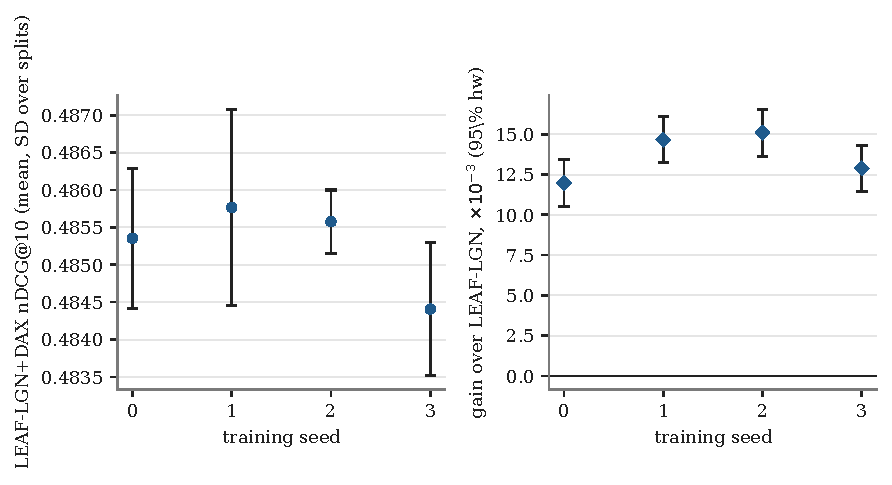
\includegraphics[width=0.85\linewidth]{figs/fig_seeds.pdf}
\caption{Training seeds 0 to 3 on KuaiRand-27K. Left: LEAF-LGN+DAX mean nDCG@10 with the standard deviation over splits. Right: within-seed gain over LEAF-LGN with the 95\% half-width. Source: \texttt{results/v11/dax\_lgn\_post.json} (seed 0) and \texttt{results/v11/c\_seeds/lgn\_s1.json} to \texttt{lgn\_s3.json}.}
\label{fig:seeds}
\end{figure}

\begin{table}[tbp]
\centering
\footnotesize
\caption{Training seeds on KuaiRand-27K: LEAF-LGN+DAX and its within-seed gain over LEAF-LGN (same seed), seeds 0 to 3.}
\label{tab:seeds}
\begin{adjustbox}{max width=\linewidth}
\begin{tabular}{lrrrccc}
\toprule
Seed & LEAF-LGN+DAX & LEAF-LGN & Configs & Gain [95\% hw] & $p$ & NB $p$ \\
\midrule
0 (main run) & 0.4854 & 0.4736 & 3840 & +11.96 [1.47] & $6.55\times10^{-57}$ & 0.001 \\
1 & 0.4858 & 0.4714 & 640 & +14.67 [1.42] & $1.63\times10^{-90}$ & 0.001 \\
2 & 0.4856 & 0.4708 & 640 & +15.10 [1.46] & $1.87\times10^{-90}$ & 0.002 \\
3 & 0.4844 & 0.4716 & 640 & +12.89 [1.44] & $1.90\times10^{-68}$ & 0.002 \\
\midrule
Spread over seeds & 0.4853 $\pm$ 0.0006 &  &  & +13.65 $\pm$ 1.48 &  &  \\
QP family (seeds not run) & \textnormal{\{TBD:results/v11/c\_seeds QP seeds 1-3: qp\_s1.json.partial.json incomplete\}} &  &  &  &  &  \\
\bottomrule
\end{tabular}
\end{adjustbox}
\par\smallskip
\begin{minipage}{\linewidth}\raggedright\footnotesize Seed 0 is the main run with the full backbone grid (12 trainings). Seeds 1 to 3 re-train with the training seed changed and a reduced backbone grid: lr 3e-3 and wd 1e-4 in every split, w in {0.25, 0.5} for the DAX arm (2 trainings) and w 0.25 for the base. The epoch, the DAX configuration and gamma are selected on validation per split. Raw p values, not Holm-adjusted. The QP family was not re-trained under seeds 1 to 3, so no seed comparison with it is reported.\end{minipage}
\end{table}


\subsection{Lifelong deep baselines}\label{sec:res-deep}

DIN attends over the last 200 lifelong events of each user. On KuaiRand-27K it reaches 0.4675 and is below LEAF-LGN+DAX by $+18.26$ [1.97] (per-user t test, Holm-adjusted $p=5.62\times10^{-73}$). DIN with DAX reaches 0.4796 and remains below LEAF-LGN+DAX by $+5.73$ [1.64] (Holm-adjusted $p=7.95\times10^{-12}$; Nadeau-Bengio Holm-adjusted $p=4.56\times10^{-2}$). SIM-hard, which keeps the 50 most recent events that share the candidate's tag or author, has no KuaiRand-27K result file yet, so its rows are pending. On KuaiRand-1K, LEAF-LGN+DAX (0.4590) is above DIN with DAX (0.4228) and above SIM-hard (0.4246) and SIM with DAX (0.4357); the unadjusted differences are reported in Table~\ref{tab:deep}. The deep models are tuned over four configurations each (learning rate and weight decay, with the DAX arms on the post-hoc grid), so they are not tuned as widely as LEAF-LGN. The paper does not claim that LEAF-LGN+DAX is better than a lifelong deep model that has been tuned over a wider grid.

\begin{table}[tbp]
\centering
\footnotesize
\caption{Lifelong deep baselines (DIN and SIM-hard) with and without DAX, and their paired difference to LEAF-LGN+DAX (LEAF-LGN+DAX minus the comparator, x1e-3 nDCG@10).}
\label{tab:deep}
\begin{adjustbox}{max width=\linewidth}
\begin{tabular}{lrccccc}
\toprule
Comparator & Mean & Configs & Diff.\ [95\% hw] & $p$ & NB $p$ \\
\midrule
\multicolumn{6}{l}{KuaiRand-27K} \\
DIN & 0.4675 & 4 & +18.26 [1.97] & $1.41\times10^{-73}$ & 0.001 \\
DIN+DAX & 0.4796 & 1280 & +5.73 [1.64] & $7.95\times10^{-12}$ & 0.043 \\
SIM & \textnormal{\{TBD:results/v12/sim\_27k.json SIM mean\}} & \textnormal{\{TBD:results/v12/sim\_27k.json SIM configs\}} & \textnormal{\{TBD:results/v12/sim\_27k.json SIM difference\}} &  &  \\
SIM+DAX & \textnormal{\{TBD:results/v12/sim\_27k.json SIM+DAX mean\}} & \textnormal{\{TBD:results/v12/sim\_27k.json SIM+DAX configs\}} & \textnormal{\{TBD:results/v12/sim\_27k.json SIM+DAX difference\}} &  &  \\
\midrule
\multicolumn{6}{l}{KuaiRand-1K} \\
DIN & 0.4189 & 4 & +39.26 [10.37] & $2.63\times10^{-13}$ & 0.002 \\
DIN+DAX & 0.4228 & 1280 & +35.89 [9.25] & $7.10\times10^{-14}$ & 0.002 \\
SIM & 0.4246 & 4 & +35.26 [9.24] & $1.70\times10^{-13}$ & 0.007 \\
SIM+DAX & 0.4357 & 1280 & +23.29 [8.69] & $1.81\times10^{-7}$ & 0.095 \\
\midrule
\multicolumn{6}{l}{Lifelong sequence models: DIN attends over the last 200 lifelong events; SIM-hard keeps the 50 most recent events sharing the candidate's tag or author.} \\
\bottomrule
\end{tabular}
\end{adjustbox}
\par\smallskip
\begin{minipage}{\linewidth}\raggedright\footnotesize Raw p values. DIN and SIM are tuned over four configurations (lr {1e-2, 3e-3} times wd {1e-4, 1e-5}) with patience 2; their +DAX arms use the post-hoc DAX grid. Entries marked TBD have no result file yet.\end{minipage}
\end{table}


\subsection{What the controls show}\label{sec:res-controls}

The LEAF controls come from the stage 1 run on the LEAF-tied backbone, the closed-form variant on which those ablations were run (Table~\ref{tab:leafctl}). Shuffling the users' lifelong tables across users gives the largest loss, $+18.90$ [1.99] (Holm-adjusted $p=4.90\times10^{-76}$; Nadeau-Bengio Holm-adjusted $p=4.60\times10^{-3}$), and removing all lifelong channels gives $+17.88$ [2.04]. The design check of that run, the difference between the shuffled-user arm and the no-lifelong arm, is $-1.02\times10^{-3}$, within its $\pm2\times10^{-3}$ tolerance. The policy channel contributes $+5.01$ [1.20] (per-user t test Holm-adjusted $p=6.91\times10^{-16}$), but its split-level test is not significant after Holm adjustment (Nadeau-Bengio Holm-adjusted $p=0.132$). The LEAF-LGN ablations have no result file (\texttt{results/v10/leaf\_lgn\_ablate.json} is missing), so the controls are reported on the LEAF-tied backbone only.

\begin{table}[tbp]
\centering
\footnotesize
\caption{LEAF controls on KuaiRand-27K (stage 1 stored run, LEAF-tied backbone): arm means and full minus arm.}
\label{tab:leafctl}
\begin{adjustbox}{max width=\linewidth}
\begin{tabular}{lrccccc}
\toprule
Arm & Configs & Mean & Full minus arm [95\% hw] & $p_{\mathrm{Holm}}$ & NB $p$ & NB $p_{\mathrm{Holm}}$ \\
\midrule
LEAF-tied (full) & 3456 & 0.4691 & n/a & n/a & n/a & n/a \\
\midrule
shuffle users & 3456 & 0.4499 & +18.90 [1.99] & $4.90\times10^{-76}$ & 0.001 & $4.60\times10^{-3}$ \\
no tag channels & 1152 & 0.4594 & +9.38 [1.63] & $1.17\times10^{-28}$ & 0.002 & $6.48\times10^{-3}$ \\
no author channels & 432 & 0.4628 & +6.45 [1.17] & $2.10\times10^{-26}$ & 0.001 & $4.42\times10^{-3}$ \\
no lifelong channels & 72 & 0.4512 & +17.88 [2.04] & $9.61\times10^{-65}$ & 0.000 & $2.51\times10^{-3}$ \\
no policy channel & 864 & 0.4643 & +5.01 [1.20] & $6.91\times10^{-16}$ & 0.066 & $1.32\times10^{-1}$ \\
lift only & 432 & 0.4634 & +5.78 [1.11] & $6.10\times10^{-24}$ & 0.001 & $4.60\times10^{-3}$ \\
familiarity only & 576 & 0.4585 & +10.26 [1.66] & $4.07\times10^{-33}$ & 0.001 & $4.60\times10^{-3}$ \\
no music channels & 1728 & 0.4691 & 0.00 [0.00] & 1 & 1.000 & 1 \\
\bottomrule
\end{tabular}
\end{adjustbox}
\par\smallskip
\begin{minipage}{\linewidth}\raggedright\footnotesize Full minus arm: positive means the channel helps. Holm within the eight arms; NB over the split means. The no-music arm gives identical rankings in every split. The LEAF-LGN ablations are not run (results/v10/leaf\_lgn\_ablate.json is missing); these controls use the closed-form LEAF-tied backbone. The shuffle-users control removes the lifelong gain (design check on the difference between the shuffled and the no-lifelong arm).\end{minipage}
\end{table}


\subsection{Summary of the evidence}\label{sec:res-summary}

Across the controls the picture is consistent. The LEAF signal depends on the users' lifelong histories and not only on the item channels: shuffling the users removes the gain. The DAX module depends on the item-level appeal beyond the tag mean and on its user and scenario terms, and a shuffle across items removes its gain. The combination is above every comparator with a result, including the lifelong deep models with DAX on KuaiRand-27K and KuaiRand-1K, and its gain is not specific to one training seed or to the 1K subset. The controls do not establish that the item-level estimate is an unbiased measure of item quality; Section~\ref{sec:limits} lists what remains untested.
